% (c) Egor Osipov

\documentclass[a4paper,12pt]{article} % тип документа (report, book)
\usepackage[14pt]{extsizes}
\usepackage[left=2cm,right=2cm, top=2cm,bottom=2cm,bindingoffset=0cm]{geometry} % Настройки документа
\usepackage{pgfplots}
\usepackage{pgfplotstable}
\usepackage{tikz} 

%  Русский язык
\usepackage[T2A]{fontenc}			% кодировка
\usepackage[utf8]{inputenc}			% кодировка исходного текста
\usepackage[english,russian]{babel}	% локализация и переносы


% Математика
\usepackage{amsmath,amsfonts,amssymb,amsthm,mathtools} 

% Просто смайлики
\usepackage{wasysym}

%Вставка картинок
\usepackage{graphicx}
\graphicspath{./}
\DeclareGraphicsExtensions{.pdf,.png,.jpg}
\usepackage{float}

% Настройка абзацев
\usepackage{indentfirst}
%\setlength{\parindent}{5ex}
%\setlength{\parskip}{1em}

\begin{document} % начало документа

%Заговолок
\begin{titlepage}
\begin{center}
	\large{Московский физико-технический институт}\\
	\vspace{100px}
	\LARGE{Лабораторная работа № 3.4.1.}\\
	\LARGE{Диа- и парамагнетики.}\\
	\vspace{30px}
	
\includegraphics[scale = 0.3]{fakt_logo.png}\\
\end{center}

\vfill
\begin{flushright}
	\text{Осипов Егор. Б03-005}\\
	\text{22.09.2021}\\
	\text{г. Долгопрудный}
\end{flushright}
\end{titlepage}

\newpage

\tableofcontents

\newpage

\section{Цель работы и инструменты.}

\textbf{Цель работы:} Измерение магнитной восприимчивости диа- и парамагнитного образца.

\textbf{В работе используются:} электромагнит, аналитические весы, миливеберметр, амперметр постоянного тока, реостаты, образцы.

\section{Подготовка к работе.}

\subsection{Теоритические выкладки}

Магнитная восприимчивость тел может быть определена мегодом измерения сил, которые действуют на тела в магнитном поле. Существуют два классических метода таких измерений: \textit{метод Фарадея} и \textit{метод Гюи}. В методе Фарадея исследуемые образцы, имеющие форму маленьких шариков, помещаются в область сильно неоднородного магнитного поля и измеряется сила, действующая на образец. При этом для расчёта магнитной восприимчивости необходимо знать величину градиента магнитного поля в месте расположения образца. В методе Гюи используется тонкий и длинный стержень, один из концов которого помещают в зазор электромагнита (обычно в область однородного поля), а другой конец — вне зазора, где величиной магнитного поля можно пренебречь. Закон изменения поля — от максимального до нулевого — в этом случае несуществен.

Найдём выражение для магнитной силы, действующей на такой образец (рис. \eqref{pic1}). Пусть площадь образца равна в, его магнитная проницаемость — р, а поле в зазоре равно В.

\begin{figure}[H]\label{pic1}
	\center{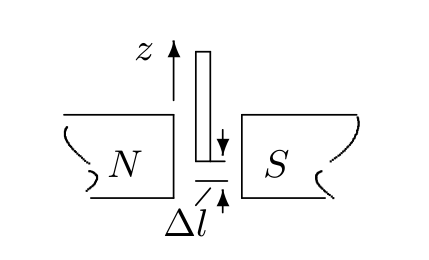
\includegraphics[scale=0.4]{pic1}}
	\caption{Расположение образца в зазоре электромагнита}
\end{figure}

Воспользуемся для расчёта энергетическими соображениями. Магнитная сила может быль вычислена как производная от магнитной энергии по
перемещению. Из теории известно, что эту производную следует брать со знаком минус, когда образец находится в поле постоянного магнита, или со знаком плюс, как в нашем случае, когда поле в зазоре создаётся электромагнитом, ток I в обмолках которого поддерживается постоянным

При смещении образца на расстояние $\vartriangle l$ вниз магнитная сила, действующая на него равна:

\begin{equation}\label{eq1}
F = (\frac{\vartriangle W_m}{\vartriangle l})
\end{equation}
где $\vartriangle W_m$ -- изменение магнитной энергии системы при постоянном токе в обмотке электромагнита и, следовательно, при постоянной величине магнитного поля в зазоре.

Магнитная энергия рассчитывается по формуле:

\begin{equation}\label{eq2}
W_m = \frac{1}{2} \int HBdV = \frac{1}{2\mu_0} \int \frac{B^2}{\mu} dV
\end{equation}
где интеграл распространён на всё пространство. При смещении образца магнитная энергия меняется только в области зазора (в объёме илощади в и высоты $\vartriangle l$), а около верхнего конца стержня остаётся неизменной, поскольку магнитного поля там практически нет. Принимая поле
внутри стержня равным измеренному нами полю в зазоре В, получим:

\begin{equation*}
\vartriangle W_m = \frac{1}{2\mu_0} \frac{B^2}{\mu} s \vartriangle l
- \frac{1}{2\mu_0} B^2 s \vartriangle l = \frac{1 - \mu}{2\mu_0 \mu} B^2 s \vartriangle l = - \frac{\chi}{2 \mu_0 \mu} B^2 s \vartriangle l
\end{equation*}

Следовательно на образец действует сила:

\begin{equation}\label{eq3}
F = - \frac{\chi}{2 \mu_0 \mu} B^2 s
\end{equation}
Знак силы, действующей на образец, зависит от знака  $\chi$: образцы из парамагнитных материалов ($\chi$ > 0) втягиваются в зазор электромагнита,
а диамагнитные образцы ($\chi$ < 0) выталкиваются из него.

Пренебрегая отличием и от единицы, получаем окончательно расчётную формулу в виде:

\begin{equation}\label{eq4}
F = - \frac{\chi B^2 s}{2 \mu_0}
\end{equation}

Измерив силу, действующую на образец в магнитном поле B, можно рассчитать магнитную восприимчивость образца.

\subsection{Экспериментальная установка.}

\begin{figure}[H]\label{pic2}
	\center{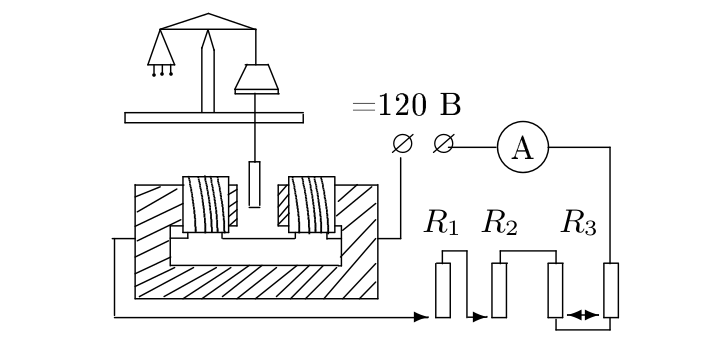
\includegraphics[scale=0.4]{pic2}}
	\caption{Схема экспериментальной установки.}
\end{figure}

Схема установки изображена на рис. \eqref{pic2}. Магнитное поле с максимальной индукцией $\simeq$1,5 Тл создаётся в зазоре электромагнита, питаемого постоянным током. Диаметр полюсов существенно превосходит ширину зазора, поэтому поле в средней части зазора достаточно однородно. Величина тока, проходящего через обмотки электромагнита, регулируется при помощи трёх реостатов $R_1$, $R_2$, $R_3$ и измеряется многопредельным амперметром А. Тонкая проволока высокоомных реостатов не рассчитана на большой ток, поэтому регулировку более низкоомными реостатами следует проводить только при \textbf{полностью} выведенных высокоомных реостатах.

Градуировка электромагнита, (связь между индукцией магнитного поля В в зазоре электромагнита, и силой тока I в его обмотках) производится при помощи милливеберметра (описание милливеберметра и правила работы с ним приведены на с. 138).

При измерениях образцы поочерёдно подвешиваются к аналитическим весам так, что один конец образца оказывается в зазоре электромагнита, а другой — вне зазора, где индукцией магнитного поля можно пренебречь. При помощи аналитических весов определяется перегрузка $\vartriangle P = F$ -- сила, действующая на образец со стороны магнитного поля.

Как уже отмечалось, силы, действующей на диа- и парамагнитные образцы, очень малы. Небольшие примеси ферромагнетиков (сотые доли процента железа или никеля) способны кардинально изменить результат опыта, поэтому образцы были специально отобраны.

\section{Ход работы.}

В работе предлагается исследовать зависимость силы, действующей на образец, размещённый в зазоре электромагнита, от величины поля в зазоре и по результатам измерений рассчитать магнитную восприимчивость меди и алюминия.\\
1. Проверьте работу цепи питания электромагнита. Оцените диапазон
изменения тока I через обмотки.\\
2. Прокалибруйте электромагнит. Для этого с помощью милливебермет-
ра снимите зависимость магнитного потока $\Phi$, пронизывающего проб-
ную катушку, находящуюся в зазоре, от тока I ($\Phi$ = BSN). Значение
SN (произведение площади сечения пробной катушки на число витков
в ней) указано на установке.

\begin{center}
\textbf{Включать и отключать электромагнит следует только при минимальном токе!}
\end{center}
3. Убедимся, что весы арретированы.

\begin{center}
\textbf{Весы следует арретировать перед каждым изменением тока.}
\end{center}
4. Измерим силы, действующие на образец в магнитном поле. Для это-
го, не включая электромагнит, подвесьте к весам один из образцов.
Установите на весах примерное значение массы образца (масса, диа-
метр и максимальное значение перегрузки для каждого образца, ука-
заны на установке). Освободите весы и добейтесь точного равновесия
весов.

Арретируем весы. Установим минимальное значение тока и провеем измерение равновесного значения массы. Повторите измерения т = {(Т) для 6-8 других значений тока.

Повторим измерения $m = f(T)$ для 6-8 других значений тока.\\
5. Повторим измерения п.4 для другого образца

\end{document} % конец документа